\section{Architecture}
This chapter describes the architecture of the application. 

\subsection{Software Design Pattern}
This application is developed according to the MVC software architecture pattern. 
The MVC (Model-View-Controller) pattern, as depicted in the following diagram, is a software architectural pattern for implementing user interfaces. It divides an application into three interconnected components:

\begin{itemize}
    \item \textbf{Model:} Represents the data structure, business logic, and rules of the application. In your diagram, the model is represented by classes like FileModel, FolderModel, URLPair, and ConfigModel.
    \item \textbf{View:} Displays the data (the model) to the user and sends user commands to the controller. The ConsoleView is an example of this component in your diagram.
    \item \textbf{Controller:} Handles user input, interacts with the model, and selects the view to present. In the diagram, this is represented by CLIController.
    
\end{itemize}

The interaction between these components allows for efficient code separation, easier maintenance, and development. The Main class acts as the entry point of the application, orchestrating the MVC pattern. The Controller uses and updates the Model, and the View is also updated accordingly, maintaining a clear separation of concerns.

Below is an overview of the MVC pattern used in this application.

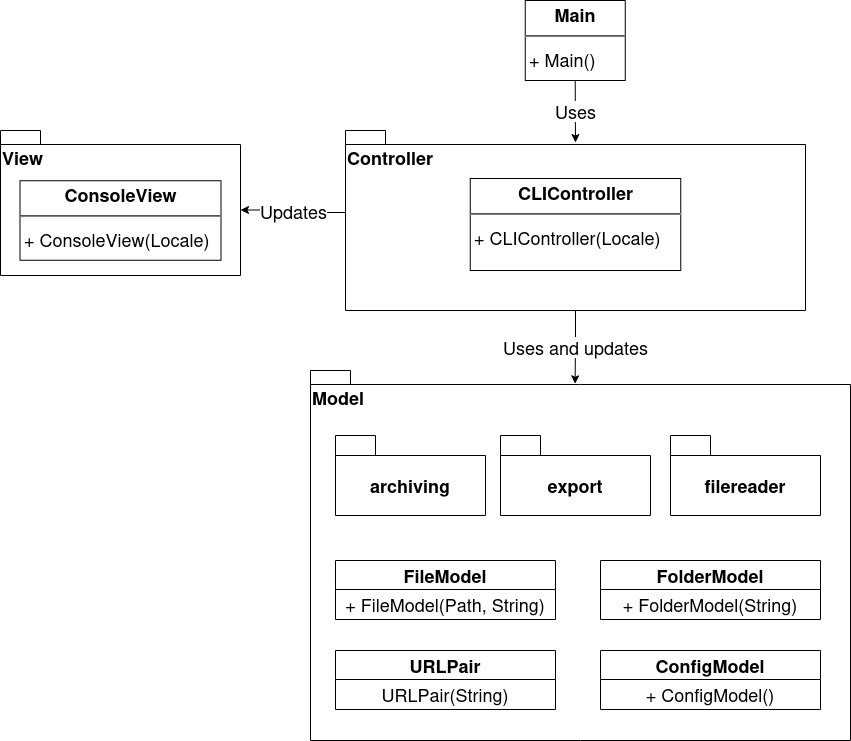
\includegraphics[width=1\textwidth]{diagrams/mvc_diagram-Highlevel_MVC.png}
\clearpage

\subsection{Factory Pattern}
In this application the factory pattern was used.
The Factory Pattern in software design is a creational pattern that provides a way to encapsulate the instantiation of objects. Instead of directly creating objects using the `new` operator, this pattern delegates the responsibility of object creation to a factory. This abstraction allows for greater flexibility and scalability in code. It's particularly useful when the exact types of objects to be created can vary or when there needs to be some logic involved in the creation of these objects. The Factory Pattern aids in maintaining a clear separation of concerns and promotes code reusability, making it a fundamental concept in object-oriented design and programming.

In the architecture of the application, two crucial factories, the `FileReaderFactory` and the `ExporterFactory`, play essential roles:

\begin{itemize}
    \item \textbf{FileReaderFactory:} This factory is responsible for creating objects that read various file types. It simplifies file handling by providing objects that adhere to the `FileReaderInterface`.
    \item \textbf{ExporterFactory:} This factory generates exporters for different data formats, offering a unified interface to obtain the appropriate data exporter.
\end{itemize}

These factories enhance the application's modularity and extensibility by encapsulating the creation logic of their respective components, thus promoting loose coupling and scalability. This approach aligns with the Factory Design Pattern principles, improving maintainability and adaptability to new file types and data export formats. \\

The following two diagrams illustrate these factories.
\clearpage

\textbf{FileReaderFactory:} \\
\vskip 0.5cm
\begin{center}
    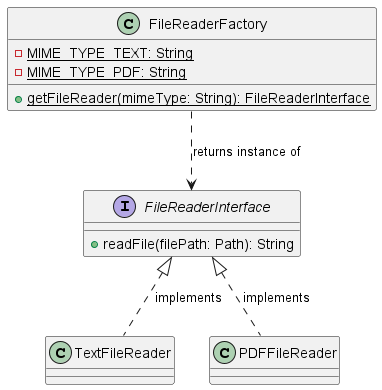
\includegraphics[width=0.6\textwidth]{pictures/FileReaderFactory-0.png}
\end{center}
\vskip 1cm
\textbf{ExporterFactory:} \\
\vskip 0.5cm
\begin{center}
    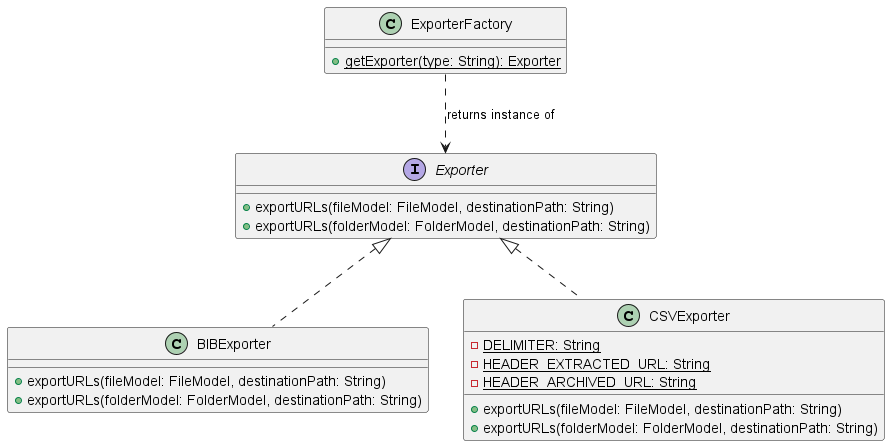
\includegraphics[width=1\textwidth]{pictures/ExporterFactory-0.png}
\end{center}

\subsection{Config File}
In this application, the use of a configuration JSON file is instrumental for managing various settings and parameters. The application includes classes like `ConfigModel` and `ConfigFileHelper` to interact with this file. `ConfigModel` defines the structure of the configuration data, ensuring that all necessary settings are represented and easily accessible within the application. `ConfigFileHelper`, on the other hand, handles the reading and writing of the JSON configuration file, abstracting these operations from the rest of the application's code. This approach not only simplifies the management of configuration settings but also enhances the application's flexibility, as changes to configuration do not require alterations in the codebase.

The config file looks like this:

\{

\quad''accessKey'':''[Access Key]'',

\quad''secretKey'':''[Secretkey]'',

\quad''browser'':''FIREFOX''

\}


The config file can be modified with the application during runtime. However, the changes can also be made directly in the file as long as the format is correct.
At the moment the application saves the credentials for the WayBackMachine and the selected brwoser for the archive.today service.
\clearpage

\subsection{Frontend}
The frontend architecture of this application is structured around a console-based interface, as indicated by the `ConsoleView` and `CLIController` classes. The `ConsoleView` class is responsible for presenting information to the user and handling user input in a console environment. It's designed to display data and messages in a clear and user-friendly manner. The `CLIController`, part of the Controller component in the MVC pattern, acts as an intermediary between the `ConsoleView` and the application's backend. It processes user inputs received through the `ConsoleView`, interacts with the model to retrieve or update data, and then reflects these changes back on the console interface. This architecture allows for a straightforward and efficient user interaction in a command-line environment.
\vskip 1cm
\begin{center}
    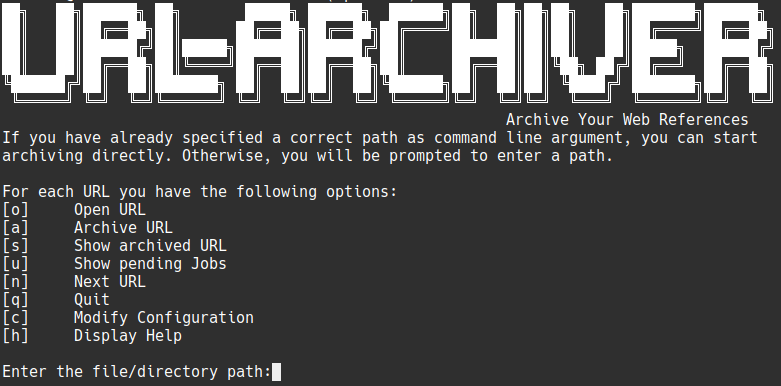
\includegraphics[width=1\textwidth]{pictures/final_presentation/command_line_application.jpg}
\end{center}



\clearpage